% Copyright (c) 2021 Eclipse Arrowhead Project
%
% This program and the accompanying materials are made available under the
% terms of the Eclipse Public License 2.0 which is available at
% http://www.eclipse.org/legal/epl-2.0.
%
% SPDX-License-Identifier: EPL-2.0

We expect the automation system of today to keep becoming more and more computerized, digitized and interconnected.
By this we mean that more aspects of and surrounding machines will be handled by computers, more information will be made available to those computers and, finally, comparatively more computers will be given the opportunity to collect, communicate and act on that information.
Manufacturing, transportation, energy distribution, medicine, recycling, and all other industrial sectors concerned with automation will be affected by this development.
It will lead to increased efficiency and flexibility, as machines become able to perform more of the work traditionally assigned to humans.
However, it will also lead to new magnitudes of complexity, not the least because of the renewed incentive to use more and more of these highly communicative machines.

The \GlossaryHyperRef{framework-arrowhead}{\textit{Arrowhead framework}} is designed to address this explosion of complexity.
It provides a foundation for \GlossaryHyperRef{communication-service-oriented}{\textit{service-oriented communication}} \cite{mackenzie2006reference} between automation systems, such that interoperability, security, safety, performance, and other major concerns can be addressed efficiently and effectively.
It notably allows for \GlossaryHyperRef{system}{system} \GlossaryHyperRef{capability}{capabilities} to be \GlossaryHyperRef{description}{described}, shared and exploited dynamically by communicating \GlossaryHyperRef{device}{devices}.

In this document, we, the Eclipse Arrowhead project, present an authoritative set of concept definitions, meant to serve as the fundamental language for discussions about and the modeling of Arrowhead-based \GlossaryHyperRef{design}{designs}.
These definitions exist to help mitigate compatibility and consistency issues in \GlossaryHyperRef{software}{software}, tooling, \GlossaryHyperRef{model}{models}, documentation and all other things of relevance to the Arrowhead framework.

\subsection{Primary Audiences}
\label{sec:introduction:audiences}

This document is being written and maintained for all who may require a precise and rigorous understanding of the Arrowhead framework, which we understand is likely to include the following groups:

\begin{itemize}
\item System \GlossaryHyperRef{designer}{designers}, \GlossaryHyperRef{engineer-standardization}{standardization engineers}, \GlossaryHyperRef{developer}{developers}, \GlossaryHyperRef{integrator}{integrators} and \GlossaryHyperRef{operator}{operators}.
\item \GlossaryHyperRef{researcher}{Researchers}.
\item Technical \GlossaryHyperRef{manager}{managers} and advanced \GlossaryHyperRef{user}{users}.
\end{itemize}

\subsection{Scope}
\label{sec:introduction:scope}

The concepts described in this document make up a so-called \GlossaryHyperRef{model-reference}{\textit{reference model}}, which we understand to be a set of definitions for technical concepts of fundamental importance to a specific problem domain.
Such a document does not specify how its definitions should be used to design systems, either abstract or concrete.
Reference models can be used as vocabularies for defining \GlossaryHyperRef{architecture-reference}{reference architectures}, which in turn can be used to derive \GlossaryHyperRef{architecture}{concrete architectures} and, finally, \GlossaryHyperRef{implementation-software}{software implementations}, as illustrated in Figure \ref{fig:reference-model}.

\begin{figure}[ht]
  \centering
  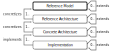
\includegraphics{figures/reference-model}
  \caption{
    The steps from reference model to implementation, going from highly abstract to entirely concrete.
    Reference models define fundamental concepts, reference architectures add abstract and/or concrete design constraints rooted in real-world observations or experiences, concrete architectures makes those design constraints practically realizable as one or more \GlossaryHyperRef{artifact}{artifacts}, while implementations represent their actual realization.
  }
  \label{fig:reference-model}
\end{figure}

\subsection{Notational Conventions}
\label{sec:introduction:conventions}

The following conventions regarding diagrams, references and requirements are adhered to throughout this document.
All three of them were selected by virtue of being deemed unsurprising to our primary audiences.

\subsubsection{Diagrams}

A box with a name inside it denotes a named \GlossaryHyperRef{entity}{entity} or \GlossaryHyperRef{stakeholder}{stakeholder}.
A named arrow between boxes denotes the \GlossaryHyperRef{relationship}{relationship} implied by the name.
If a named arrow has an associated positive integer or range, which we refer to as a \textit{quantifier}, the relation is to be considered as extending to the number of distinct entities indicated by that integer or range.
A range is denoted by $x..y$, where $x$ and $y$ are positive integers and $x<y$.
Omitting $y$ when using the range notation (e.g. ``$1..$'') means that the range is infinite from $x$.
If two or more arrows are combined such that their source or target end is shared, a difference is made if a quantifier is closest to a shared or non-shared arrow part.
If it is closest to a shared part, the quantity must be understood to apply to every arrow part of the combination.
If it is closest to a non-shared part, the quantifier must be understood to only apply to that arrow.
A box with a dotted border represents a group.
The entities explicitly placed within the box may or may not represent all entities that belong to that group.
See Figure \ref{fig:reference-model} for an example of this notation being used.

Note that this document does \textit{not} define an Arrowhead profile for SysML \cite{omg2019sysml}, or any other modeling language.
As we cover later in Section \ref{sec:conformance}, however, we do expect all models based on this document not to contradict any of its definitions.

\subsubsection{References}

Square brackets around numbers (e.g. \cite{delsing2017iot}) are references to the reference list in Section \ref{sec:references}.
The number within the brackets of any given reference corresponds to the entry with the same number in the reference list.

References within this document are hyperlinked, which means that those reading it electronically can click the references and immediately be taken to their targets.
Special treatment is given to references targeting Section \ref{sec:glossary}, the \nameref{sec:glossary}.
These are displayed as regular text rendered with blue color.

\subsubsection{Requirements}

Use of the words \textbf{must}, \textbf{must not}, \textbf{required}, \textbf{should}, \textbf{should not}, \textbf{recommended}, \textbf{may}, and \textbf{optional} are to be interpreted as follows when used in this document: \textbf{must} and \textbf{required} denote absolute requirements that must be adhered to for a described entity to be considered as compliant to this reference model; \textbf{must not} denotes an absolute prohibition; \textbf{should}, \textbf{should not} and \textbf{recommended} denote recommendations that should be deviated from only if special circumstances make it relevant; and, finally, \textbf{may} and \textbf{optional} denote something being truly optional.
These word definitions are derived from and are meant to capture what is outlined in RFC 2119 \cite{bradner1997keywords}.

\subsection{Relationships to Other Documents}
\label{sec:introduction:relationships}

When this \GlossaryHyperRef{model-reference}{reference model} was produced, care was taken to reuse or build upon the concepts presented in the following works:

\begin{enumerate}
\item \textbf{Reference Architecture Model Industrie 4.0} (RAMI4.0) \cite{adolphs2016reference}, which outlines an ontological and architectural view of \GlossaryHyperRef{industry40}{\textit{Industry 4.0}}.
The document may be seen as a predecessor to, or major influence on, the conceptual aspects of the Arrowhead framework.
In particular, the document describes how to model and design communicating industrial systems such that key Industry 4.0 characteristics can be facilitated, such as high degrees of dynamicity and interoperability.
However, as RAMI4.0 is a reference \textit{architecture} rather than a reference \textit{model}, we have only been concerned with what concepts it defines and what problems it frames.
This delimitation excludes its ``architectural layers'', ``life-cycle \& value-stream'' phases and ``hierarchical levels'', as well as the abstract design of its ``asset administrative shell''.
These excluded aspects are neither condemned nor endorsed by this document.
They are simply outside its scope.

\item \textbf{Reference Model for Service Oriented Architecture} (SOA-RM) \cite{mackenzie2006reference}, which provides a standardized definition of Service-Oriented Architecture (SOA).
As communication between \GlossaryHyperRef{system}{systems} of the Arrowhead framework is understood to follow this paradigm, it becomes particularly relevant to consider.

\item \textbf{IoT Automation: Arrowhead Framework} (IoTA:AF) \cite{delsing2017iot}, which significantly includes an overview of the \textit{local automation cloud} concept in its second chapter, as well as the \textit{Arrowhead framework architecture} in its third chapter.
The book most significantly represents the state of the Arrowhead framework up until it was written.
Even though the framework has evolved since then, it still represents the most comprehensive view of the framework.
While the strictly architectural aspects of IoTA:AF are outside the scope of this document, the two mentioned chapters contain several definition with a high degree of relevance.

\end{enumerate}

Only conformity with IoTA:AF is observed strictly, which means that concept definitions presented here may diverge from those of the other two works.
All significant terminology differences are noted in the glossary of Section \ref{sec:glossary}, which briefly defines all concepts of relevance to this document.

\subsection{Section Overview}
\label{sec:introduction:sections}

The remaining sections of this document are organized as follows:
\vspace*{2mm}
\begin{itemize}[leftmargin=2cm,rightmargin=0pt,labelwidth=2cm,labelsep=0pt,itemindent=0pt,parsep=0.1cm,topsep=0.1cm,align=left]

\item[Section \ref{sec:introduction}]
This section.

\item[Section \ref{sec:arrowhead}]
An informal overview of Arrowhead, serving both to provide a workable summary of the framework and to prepare readers for better understanding Section \ref{sec:model}.

\item[Section \ref{sec:model}]
The formal and normative description of Arrowhead.
Each of its subsections is concerned with one major Arrowhead concept, ranging from entities to systems-of-local-clouds.

\item[Section \ref{sec:conformance}]
A brief list of requirements, meant to help determine whether or not a given model or document is conforming to this reference model.

\item[Section \ref{sec:glossary}]
Lists all significant terms and abbreviations presented in this document in alphabetical order.

\item[Section \ref{sec:references}]
Lists references to publications referred to in this document.

\item[Section \ref{sec:revision}]
Records the history of changes made to this document.

\end{itemize}
